\documentclass[a4paper,10pt]{article}
\usepackage[utf8]{inputenc}

\usepackage[margin=1in,includefoot,footskip=30pt]{geometry}
\usepackage{tikz}
\usepackage{bbm}
\usepackage{amsmath}
\usepackage{hyperref}

\newcommand\D{\mathrm{d}}
\newcommand\R{\mathbbm{R}}

\newcommand\Convolution{\ast}
\newcommand\Correlation{\star}

\newcommand\Reversed[1]{\overline{#1}}
\newcommand\Indicator[1]{\mathbbm{1}_{#1}}

\DeclareMathOperator{\nzd}{nzd}
\DeclareMathOperator{\IntervalLeft}{left}
\DeclareMathOperator{\IntervalRight}{right}
\DeclareMathOperator{\IntervalCenter}{center}

%%%%%%%%%%%%%%%%%%%%%%%%%%%%%%%%%%%%%%%%%%%%%%%%%%%%%%%%%%%%%%%%%%%%%%%%%%%%%%%
\title{Convolution formulas using shapes}
\author{Francois Gindraud}
\date{V3}
\begin{document}
\maketitle

Formulas for convolutions are very quickly unwieldy, especially if the functions being convoluted are defined by parts.
This document shows the \emph{shape} approach to convolutions: functions are decomposed into simple geometrical shapes, and convolution of the functions are defined by combining the convolutions of simple shapes.

Pros:
\begin{itemize}
    \item Manipulate only small formulas for each shape.
    \item Individual shape convolution formulas are easier to check than huge flat formulas with lots of min/max.
    \item More readable implementation of formulas into code.
    \item High level simplifications are easier to detect if some shapes cancel with others.
\end{itemize}
Cons:
\begin{itemize}
    \item Missed simplification opportunities, if the simplifications only happen between the formulas of different shapes.
    \item More verbose than the flat strategy.
\end{itemize}

%%%%%%%%%%%%%%%%%%%%%%%%%%%%%%%%%%%%%%%%%%%%%%%%%%%%%%%%%%%%%%%%%%%%%%%%%%%%%%%
\section{Notations}

\paragraph{Convolution}
Convolution is noted using the $\Convolution$ operator, with the usual definition:
\[ \left[ f \Convolution g \right](x) = \int_\R f(x - t) g(t) \D t \]
Convolution is commutative and associative.

\paragraph{Time shift / translation}
The time shift combinator of shift $h$ moves the shape $f$ forward along the time axis by $h$.
For a shape $f$ "centered" on $c$, $\tau_h f$ is centered on $c+h$.
\[ \tau_h f(x) = f(x - h) \]
Time shifts combine additively:
\[ \tau_h (\tau_{h'} f) = \tau_{h+h'} f \]
Convolution of shifted functions is the shift of convolutions:
\[
    \left[ \tau_h f \Convolution g \right](x) =
    \int f((x - t) - h) g(t) \D t =
    \left[ f \Convolution g \right](x-h) =
    [\tau_h (f \Convolution g)](x)
\]

\paragraph{Scaling}
The scaling combinator scales the shape $f$ by a factor $c$ on the vertical axis.
\[ \left[ c \times f \right] (x) = c \times f(x) \]
Scaling combines multiplicatively with itself, and can be swapped with time shift:
\[ c \times (c' \times f) =  (c \times c') \times f \]
\[ c \times (\tau_h f) = \tau_h (c \times f) \]
Convolution of scaled functions is a scaled convolution:
\[ (c \times f) \Convolution g = c \times (f \Convolution g) \]

\paragraph{Time inversion}
A \emph{reversed} function is the shape mirrored by the vertical axis:
\[ \Reversed{f}(x) = f(-x) \]
Simplifications:
\[ \Reversed{\Reversed{f}} = f \]
\[ \Reversed{c \times f} = c \times \Reversed{f} \]
\[ \Reversed{\tau_h f}(x) = [\tau_h f](-x) = f(-x-h) = \Reversed{f}(x+h) = [\tau_{-h} \Reversed{f}] (x) \]
Convolution:
\[
    \Reversed{f \Convolution g}(x) = \int f(-x-t) g(t) \D t = \int f(-x+T) g(-T) \D T = \left[ \Reversed{f} \Convolution \Reversed{g} \right] (x)
\]

\paragraph{Sum}
The sum combinator sums the value of multiple shapes.
\[ [f+g](x) = f(x) + g(x) \]
Distributes with most operations:
\[ f \Convolution (g + h) = f \Convolution g + f \Convolution h \]
\[ \tau_s (f + g) = \tau_s f + \tau_s g \]
\[ \Reversed{f + g} = \Reversed{f} + \Reversed{g} \]

\paragraph{Cross-correlation}
Cross correlation is noted using the $\Correlation$ operator, with the usual definition:
\[ \left[ f \Correlation g \right] (x) = \int_\R f(t-x) g(t) \D t \]

It can be expressed using the convolution:
\[ \left[ f \Correlation g \right] (x) = \int \Reversed{f}(x-t) g(t) \D t = \left[ \Reversed{f} \Convolution g \right] (x) \]

Not commutative:
\[
    g \Correlation f = \Reversed{g} \Convolution f = \Reversed{\Reversed{f}} \Convolution \Reversed{g} =
    \Reversed{\Reversed{f} \Convolution g} = \Reversed{f \Correlation g}
\]

Relation with shifting is simple but not symmetric:
\[
    \tau_h f \Correlation g = \Reversed{\tau_h f} \Convolution g = \tau_{-h} \Reversed{f} \Convolution g =
    \tau_{-h} (\Reversed{f} \Convolution g) = \tau_{-h} (f \Correlation g)
\]
\[ f \Correlation \tau_h g = \Reversed{f} \Convolution \tau_h g = \tau_h (\Reversed{f} \Convolution g) = \tau_h (f \Correlation g) \]

\paragraph{Interval operations}
For interval $I = [a,b]$:
\[ h \in \R \quad I + h = h + I = [a + h, b + h] \]
\[ -I = [-b, -a] \]
\[ \IntervalLeft(I) = a \qquad \IntervalCenter(I) = \frac{a+b}{2} \qquad \IntervalRight(I) = b \]

%%%%%%%%%%%%%%%%%%%%%%%%%%%%%%%%%%%%%%%%%%%%%%%%%%%%%%%%%%%%%%%%%%%%%%%%%%%%%%%
\section{Basic shapes}

\paragraph{Indicator function}

The \emph{indicator function} for an interval $I = [a,b]$ is a rectangle of height $1$, horizontally from $a$ to $b$.
The interval can also have open bounds, changing the function value at the bounds, but not the overall shape.
\begin{center}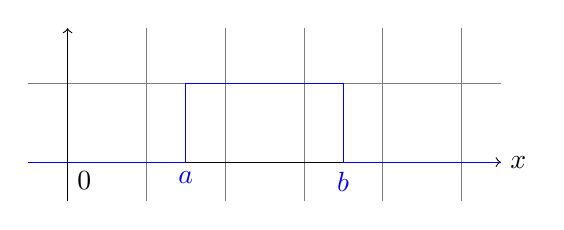
\begin{tikzpicture}
    \draw[very thin,color=gray] (-0.5, -0.5) grid (5.5, 1.7);
	\draw[->] (-0.5,0) -- (5.5,0) node[right] {$x$};
	\draw[->] (0,-0.5) -- (0, 1.7);
	\node[below right] at (0, 0) {$0$};
    \begin{scope}[color=blue]
        \draw (-0.5,0) -- (1.5,0) coordinate(a) -- (1.5,1) -- (3.5,1) -- (3.5,0) coordinate(b) -- (5.5,0);
        \node[below] at (a) {$a$};
        \node[below] at (b) {$b$};
    \end{scope}
\end{tikzpicture}\end{center}
\[
    \Indicator{[a,b]}(x) = \begin{cases}
        1 & x \in \left[ a, b \right] \\
        0 & \text{otherwise}
    \end{cases}
\]

\[ \Reversed{\Indicator{[a,b]}}(x) = \Indicator{[a,b]}(-x) = \Indicator{[-b, -a]}(x) \]
\[ \tau_h \Indicator{[a,b]}(x) = \Indicator{[a,b]}(x - h) = \Indicator{[a + h, b + h]}(x) = \Indicator{[a,b] + h}(x) \]

\paragraph{Polynom fragment}

A \emph{polynom fragment} is function whose value is a polynom on a interval $I$, and $0$ elsewhere.
The polynom itself is defined with an origin at the center of $I$ : this choice is designed to reduce floating point errors during computation, as the polynom will be evaluated "as close to its zero" as feasible.
\begin{center}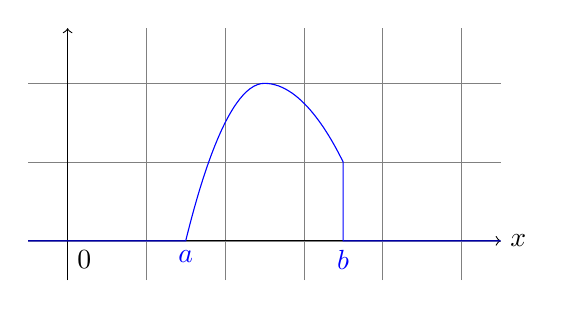
\begin{tikzpicture}
    \draw[very thin,color=gray] (-0.5, -0.5) grid (5.5, 2.7);
	\draw[->] (-0.5,0) -- (5.5,0) node[right] {$x$};
	\draw[->] (0,-0.5) -- (0, 2.7);
	\node[below right] at (0, 0) {$0$};    \begin{scope}[color=blue]
        \draw (-0.5,0) -- (1.5,0) coordinate(a) parabola[bend at end] (2.5,2) parabola (3.5,1) -- (3.5,0) coordinate(b) -- (5.5,0);
        \node[below] at (a) {$a$};
        \node[below] at (b) {$b$};
    \end{scope}
\end{tikzpicture}\end{center}
\[
    P_{I,a}(x) = \begin{cases}
        \sum_{0 \le k \le N_a} a_k (x - \IntervalCenter(I))^k & x \in I \\
        0 & \text{otherwise}
    \end{cases}
\]

Shifting does not change coefficients:
\[ \begin{split}
    \tau_h P_{I,a}(x)
    &= \sum_{0 \le k \le N_a} a_k ((x - h) - \IntervalCenter(I))^k \qquad x - h \in I \\
    &= \sum_{0 \le k \le N_a} a_k (x - (h + \IntervalCenter(I)))^k \qquad x \in I + h \\
    &= \sum_{0 \le k \le N_a} a_k (x - \IntervalCenter(I + h))^k \qquad x \in I + h \\
    &= P_{I + h, a}(x)
\end{split} \]

Reversion inverses the interval and odd coefficients:
\[ \begin{split}
    \Reversed{P_{I,a}}(x)
    &= \sum_{0 \le k \le N_a} a_k (-x - \IntervalCenter(I))^k \qquad -x \in I \\
    &= \sum_{0 \le k \le N_a} a_k (-(x - \IntervalCenter(-I)))^k \qquad x \in -I \\
    &= \sum_{0 \le k \le N_a} a_k (-1)^k (x - \IntervalCenter(-I))^k \qquad x \in -I \\
    &= P_{-I, (a_k (-1)^k)_{0 \le k \le N_a}}(x)
\end{split} \]

An indicator is a subcase of polynomial:
\[ \Indicator{I} = P_{I, a} \text{ with } (a_k) = \{a_0 = 1\} \]

%%%%%%%%%%%%%%%%%%%%%%%%%%%%%%%%%%%%%%%%%%%%%%%%%%%%%%%%%%%%%%%%%%%%%%%%%%%%%%%
\section{Polynomial Convolution \& Cross-correlation}

Convolution and cross correlation are defined on polynom fragments, which covers a lot of cases.
In particular it covers indicator functions which are polynom fragments of degree $0$.

\subsection{Convolution}

The target is to compute
\[
    C = P_{I_a,a} \Convolution P_{I_b,b}
\]
for $(a_k)_{0 \le k \le N_a}$ and $(b_j)_{0 \le j \le N_b}$.
The polynoms can be expressed as a translation of 0-centered polynoms, and thus we only need to compute convolution for 0-centered polynoms:
\[
    P_{I_a,a} = \tau_{s_a} P_{[-w_a,w_a],a}
\]
\[
    C = \tau_{s_a + s_b} (P_{[-w_a,w_a],a} \Convolution P_{[-w_b,w_b],b})
\]
In the following paragraphs the shifting $s_a + s_b$ is ignored for simplicity ; it is applied to all 3 polynom fragments result of the convolution.
We also suppose that $w_b \le w_a$ by using the commutativity of the convolution.
\[ \begin{split}
    C(x)
    &= \left[ P_{[-w_a,w_a],a} \Convolution P_{[-w_b,w_b],b} \right](x) \\
    &= \int P_{[-w_a,w_a],a}(x-t) P_{[-w_b,w_b],b}(t) \D t \\
    &= \int\limits_{\substack{x - t \in [-w_a,w_a] \\ t \in [-w_b,w_b]}} \left( \sum_{0 \le k \le N_a} a_k (x-t)^k \right) \left( \sum_{0 \le j \le N_b} b_j t^j \right) \D t \\
    &= \int\limits_{t \in [x-w_a,x+w_a] \cap [-w_b,w_b]} \left( \sum_{0 \le i \le k \le N_a} a_k \binom{k}{i} x^{k-i} (-t)^i \right) \left( \sum_{0 \le j \le N_b} b_j t^j \right) \D t \\
    &= \int\limits_{t \in I(x)} \sum_{\substack{0 \le i \le k \le N_a \\ 0 \le j \le N_b}} a_k b_j \binom{k}{i} (-1)^i x^{k-i} t^{i+j} \D t \\
    &= \sum_{\substack{0 \le i \le k \le N_a \\ 0 \le j \le N_b}} a_k b_j \binom{k}{i} (-1)^i x^{k-i} \int\limits_{I(x)} t^{i+j} \D t \\
    &= \sum_{\substack{0 \le i \le k \le N_a \\ 0 \le j \le N_b}} a_k b_j \binom{k}{i} \frac{(-1)^i}{i+j+1} x^{k-i} \left[ t^{i+j+1} \right]^{I(x)} 
\end{split} \]

Thus the value of $C(x)$ is given by integrating a polynomial expression over an interval depending on $x$ : $I(x) = [x-w_a,x+w_a] \cap [-w_b,w_b]$.
By using $w_b \le w_a$, we can compute the value of $I(x)$ which is defined piecewise in 5 cases:
\begin{center}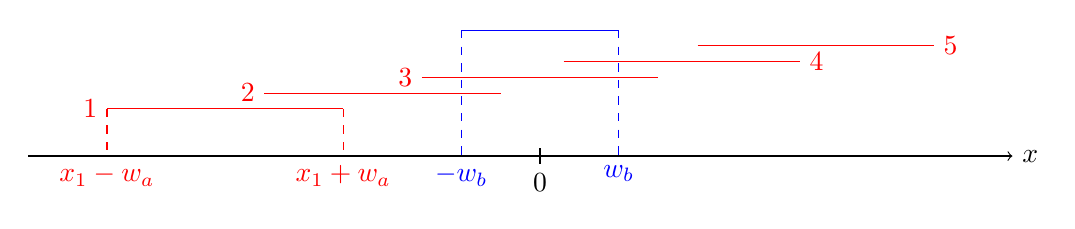
\begin{tikzpicture}
    \coordinate (Origin) at (0,0);
    \draw (0,0.1) -- (0,-0.1) node[below] {$0$};
    \draw[->] (-6.5,0) -- (6,0) node[right] {$x$};
    \begin{scope}[color=blue]
        \draw (-1,1.6) coordinate(lwq) -- +(2,0) coordinate(rwq);
        \draw[dashed] (lwq) -- (lwq |- Origin) node[below] {$-w_b$};
        \draw[dashed] (rwq) -- (rwq |- Origin) node[below] {$w_b$};
    \end{scope}
    \begin{scope}[color=red]
        \draw (-5.5,0.6) coordinate(x1l) node[left] {$1$} -- +(3,0) coordinate(x1r);
        \draw[dashed] (x1l) -- (x1l |- Origin) node[below] {$x_1-w_a$};
        \draw[dashed] (x1r) -- (x1r |- Origin) node[below] {$x_1+w_a$};
        \draw (-3.5,0.8) node[left] {$2$} -- +(3,0);
        \draw (-1.5,1) node[left] {$3$} -- +(3,0);
        \draw (0.3,1.2) -- +(3,0) node[right] {$4$};
        \draw (2,1.4) -- +(3,0) node[right] {$5$} ;
    \end{scope}
\end{tikzpicture}\end{center}
\[ I(x) = \begin{cases}
    \emptyset & x < -w_a-w_b \\
    [-w_b, x+w_a] & x \in [-w_a-w_b, -w_a+w_b] \qquad \text{"left"} \\
    [-w_b, w_b] & x \in [-w_a+w_b, w_a-w_b] \qquad \text{"center"} \\
    [x-w_a, w_b] & x \in [w_a-w_b, w_a+w_b] \qquad \text{"right"} \\
    \emptyset & x > w_a + w_b
\end{cases} \]

From the definition of $C(x)$ and the values of $I(x)$, we can determine that $C$ is defined piecewise with 3 components defined on consecutive intervals.
Moreover, as the bounds of $I(x)$ are polynomial in $x$, the 3 components are polynoms of $x$.
These 3 components are called \emph{left}, \emph{center} and \emph{right} parts.

By choosing component bounds of the form $]a,b]$, components are non-overlapping, and we have $C(x) = C_\text{left}(x) + C_\text{center}(x) + C_\text{right}(x)$.
As an additional constraint, all components are written as valid \emph{polynom fragments} : this lets us reuse the formulas to compute convolutions of convolutions like $P_1 \Convolution P_2 \Convolution P_3$.
Due to the properties of integral, $C(x)$ is continuous, and the various components must match at the border points.
This gives us some easily testable properties to check the implementations of formulas:
\[ C_\text{left}(-w_a-w_b) = 0 \]
\[ C_\text{left}(-w_a+w_b) = C_\text{center}(-w_a+w_b) \]
\[ C_\text{center}(w_a-w_b) = C_\text{right}(w_a-w_b) \]
\[ C_\text{right}(w_a+w_b) = 0 \]

\paragraph{Left part}
The left part must be of the form:
\[
	C_\text{left}(x) = P_{]-w_a-w_b, -w_a+w_b], c}(x) = \sum_k c_k (x + w_a)^k
\]
Using the integral version of $C(x)$ and the interval $I(x)$:
\[
    C_\text{left}(x) = \sum_{\substack{0 \le i \le k \le N_a \\ 0 \le j \le N_b}}
    a_k b_j \binom{k}{i} \frac{(-1)^i}{i+j+1} x^{k-i} \left( (x+w_a)^{i+j+1} - (-w_b)^{i+j+1} \right)
\]
Using binomial decomposition:
\[
	x^{k-i} = ((x+w_a) - w_a)^{k-i} = \sum_{0 \le l \le k-i} \binom{k-i}{l} (x+w_a)^{k-i-l} (-w_a)^l
\]
Injecting that into $C_\text{left}(x)$:
\[
    C_\text{left}(x) = \sum_{\substack{0 \le i \le k \le N_a \\ 0 \le j \le N_b \\ 0 \le l \le k-i}}
    a_k b_j \binom{k}{i} \binom{k-i}{l} \frac{(-1)^{i+l}}{i+j+1} w_a^l \left( (x+w_a)^{k+j+1-l} - (-w_b)^{i+j+1} (x+w_a)^{k-i-l} \right)
\]

This expression is a polynom in $x+w_a$, which was the target.
Due to its complexity, there is probably no nice closed expression for each coefficient.
However each coefficient value can be computed easily, by accumulating the factors in from of $(x+w_a)^{k+j+1-l}$ and $(x+w_a)^{k-i-l}$ for all values of $i,j,k,l$.
The degree of $C_\text{left}(x)$ is $N_a + N_b + 1$ (max of $k+j+1-l$ on the iteration space).

\paragraph{Center part}
The center part must be of the form:
\[
	C_\text{center}(x) = P_{]-(w_a-w_b), w_a-w_b], c}(x) = \sum_k c_k x^k
\]
Using the integral version of $C(x)$ and the interval $I(x)$:
\[ \begin{split}
    C_\text{center}(x)
    &= \sum_{\substack{0 \le i \le k \le N_a \\ 0 \le j \le N_b}} a_k b_j \binom{k}{i} \frac{(-1)^i}{i+j+1} x^{k-i} \left( w_b^{i+j+1} - (-w_b)^{i+j+1} \right) \\
    &= \sum_{\substack{0 \le i \le k \le N_a \\ 0 \le j \le N_b}} a_k b_j \binom{k}{i} \frac{(-1)^i}{i+j+1} w_b^{i+j+1} (1 + (-1)^{i+j}) x^{k-i}
\end{split} \]
Coefficients can be computed by accumulations as for the left part.
The degree of $C_\text{center}(x)$ is $N_a$ (max of $k-i$ on the iteration space).
As an optimisation, the computation is not done if $w_a = w_b$ as the component is $0$.

\paragraph{Right part}
The right part must be of the form:
\[
	C_\text{right}(x) = P_{]w_a-w_b, w_a+w_b], c}(x) = \sum_k c_k (x - w_a)^k
\]
Using $C(x)$ and $I(x)$ expression:
\[
    C_\text{left}(x) = \sum_{\substack{0 \le i \le k \le N_a \\ 0 \le j \le N_b}}
    a_k b_j \binom{k}{i} \frac{(-1)^i}{i+j+1} x^{k-i} \left( w_b^{i+j+1} - (x-w_a)^{i+j+1} \right)
\]
Using binomial formula, and injecting it into $C_\text{right}(x)$:
\[
	x^{k-i} = ((x-w_a) + w_a)^{k-i} = \sum_{0 \le l \le k-i} \binom{k-i}{l} (x-w_a)^{k-i-l} w_a^l
\]
\[
    C_\text{right}(x) = \sum_{\substack{0 \le i \le k \le N_a \\ 0 \le j \le N_b \\ 0 \le l \le k-i}}
    a_k b_j \binom{k}{i} \binom{k-i}{l} \frac{(-1)^i}{i+j+1} w_a^l \left( w_b^{i+j+1} (x-w_a)^{k-i-l} - (x-w_a)^{k+j+1-l} \right)
\]
This is a polynom of $x-w_a$ of degree $N_a + N_b + 1$.
As for the other parts, the coefficients can be computed by accumulation.

\subsection{Cross correlation}
The cross correlation is computed using the reverse rule:
\[ P \Correlation Q = \Reversed{P} \Convolution Q \]

The computational cost of the convolution is greater than the small reverse operation for polynomials.

\subsection{Piecewise polynoms}
This is done using distributivity of addition with respect to convolution (and cross correlation):
\[ \left[\sum_i P_i \right] \Convolution \left[\sum_j Q_j \right] = \sum_{i,j} P_i \Convolution Q_j \]

%%%%%%%%%%%%%%%%%%%%%%%%%%%%%%%%%%%%%%%%%%%%%%%%%%%%%%%%%%%%%%%%%%%%%%%%%%%%%%%
\section{Application to the Hawkes computations}
Refer to the BRP18 paper and code for details.

This section shows that various computed values are in the form :
\[ \sum_{X_l \in N_l, X_{l'} \in N_{l'}} F(X_l-X_{l'}) \]

We define the \emph{non zero domain} of a shape as an interval of $x$ containing all non zero values of $F$ : $F(x) \ne 0 \Rightarrow x \in \nzd(F)$.
This interval can be easily computed for the family of shapes and combinations introduced previously.
The sum above can then be simplified by ignoring all $X_l - X_{l'} \notin \nzd(F)$, as $F$ would be $0$.

\subsection{Base shapes used}
Basic functions considered are all piecewise polynoms

\paragraph{Histogram base}
\[ \varphi_k = \frac{1}{\sqrt{\delta}} \Indicator{\left] k\delta, (k+1)\delta \right]} \qquad 0 \le k < K \]

\paragraph{Haar wavelets}
\[ \varphi_{s,p} = \frac{\sqrt{2}^s}{\sqrt{\delta}} \left(
    \Indicator{ \left] \frac{2p \delta}{2^{s+1}}, \frac{(2p+1) \delta}{2^{s+1}} \right] } -
    \Indicator{ \left] \frac{(2p +1) \delta}{2^{s+1}}, \frac{(2p + 2) \delta}{2^{s+1}} \right] }
\right) \qquad \substack{0 \le s < \text{Nscale} \\ 0 \le p < 2^s} \]

\paragraph{Interval kernel}
\[ W_l = \frac{1}{\sqrt{\eta_l}} \Indicator{\left[ -\frac{\eta_l}{2}, \frac{\eta_l}{2} \right]} \]

\subsection{Non-kernel case}

\paragraph{B}
\[ b_{k,l}^m = \sum_{X_l \in N_l, X_m \in N_m} \varphi_k (X_m - X_l) \]

\paragraph{G}
G can be expressed as a cross correlation of phi functions:
\[ \begin{split}
    \mathsf{G}_{l,l',k,k'}
    & = \int \left( \sum_{X_l \in N_l} \varphi_k(x-X_l) \right) \left( \sum_{X_{l'} \in N_{l'}} \varphi_{k'}(x-X_{l'}) \right) \D x \\
    & = \sum_{X_l \in N_l, X_{l'} \in N_{l'}} \int \varphi_k(x-X_l) \varphi_{k'}(x-X_{l'}) \D x \\
    & = \sum_{X_l \in N_l, X_{l'} \in N_{l'}} \int \varphi_k(x-(X_l-X_l')) \varphi_{k'}(x) \D x \\
    & = \sum_{X_l \in N_l, X_{l'} \in N_{l'}} [\varphi_k \Correlation \varphi_{k'}] (X_l-X_l')
\end{split} \]

\paragraph{Penalty components}
$\widehat{V}_{k,l}^m$ is computed using a variation on the $\sum_{X_l \in N_l, X_{l'} \in N_{l'}} F(X_l-X_{l'})$ algorithm described above.
\[ \widehat{V}_{spont}^m = \int \D N_m = |N_m| \]
\[
    \widehat{V}_{k,l}^m =
    \int \left( \sum_{X_l \in N_l} \varphi_k(x-X_l) \right)^2 \D N_m =
    \sum_{X_m \in N_m} \left( \sum_{X_l \in N_l} \varphi_k(X_m-X_l) \right)^2
\]

$\widehat{B}_{k,l}^m$ is computed exactly by enumerating the values of $\sum_{X_l \in N_l} \varphi_k(x - X_l)$ for an indicator.
If $\varphi_k$ is not an indicator, we approximate it by an indicator function and use the indicator sup computation.
\[ \widehat{B}_{spont}^m = 1 \]
\[ \widehat{B}_{k,l}^m = \sup |\sum_{X_l \in N_l} \varphi_k(x - X_l)| \]

\subsection{Kernel case}

\paragraph{B}
\[ b_{W,k,l}^m = \sum_{X_l \in N_l, X_m \in N_m} [W_l \Convolution W_m \Convolution \varphi_k] (X_m - X_l) \]

\paragraph{G}
\[ \begin{split}
    \mathsf{G}_{W,l,l',k,k'}
    & = \int \left( \sum_{X_l \in N_l} [W_l \Convolution \varphi_k](x-X_l) \right) \left( \sum_{X_{l'} \in N_{l'}} [W_{l'} \Convolution \varphi_{k'}](x-X_{l'}) \right) \D x \\
    & = \sum_{X_l \in N_l, X_{l'} \in N_{l'}} \int [W_l \Convolution \varphi_k](x-X_l) [W_{l'} \Convolution \varphi_{k'}](x-X_{l'}) \D x \\
    & = \sum_{X_l \in N_l, X_{l'} \in N_{l'}} \int [W_l \Convolution \varphi_k](x-(X_l-X_l')) [W_{l'} \Convolution \varphi_{k'}](x) \D x \\
    & = \sum_{X_l \in N_l, X_{l'} \in N_{l'}} [(W_l \Convolution \varphi_k) \Correlation (W_{l'} \Convolution \varphi_{k'})] (X_l-X_l')
\end{split} \]

\paragraph{Penalty components}
TODO check expression for spontaneous cases !

\[ \widehat{V}_{W,spont}^m = \int \D N_m = |N_m| \]
\[ \widehat{V}_{W,k,l}^m = \sum_{X_m \in N_m} \left( \sum_{X_l \in N_l} [W_l \Convolution W_m \Convolution \varphi_k](X_m-X_l) \right)^2 \]

\[ \widehat{B}_{W,spont}^m = 1 \]
\[ \widehat{B}_{W,k,l}^m = \sup |\sum_{X_l \in N_l} [W_l \Convolution W_m \Convolution \varphi_k](x - X_l)| \]

\subsection{Lasso parameters}

All previous values are defined for one single region.
For multiple regions they must be combined to have only one B, G, d values.

B and G are summed over all regions:
\[ B = \sum_r B_r \]
\[ G = \sum_r G_r \]

$\widehat{V}$ is summed with a region-dependent factor.
\[ \widehat{V} = \frac{1}{R^2} \sum_r \widehat{V}_r \]

$\widehat{B}$ is summed over regions. FIXME in BRP18 the final $\widehat{B}$ is a single sup over the sum of all regions.
\[ \widehat{B} = \sum_r \widehat{B}_r \]

These two values are combined to compute $d$, coefficient wise :
\[
    d =
    \sqrt{2 \gamma \widehat{V} \log(M + M^2 K) } +
    \frac{\gamma}{3} \log(M + M^2 K) \widehat{B}
\]

%%%%%%%%%%%%%%%%%%%%%%%%%%%%%%%%%%%%%%%%%%%%%%%%%%%%%%%%%%%%%%%%%%%%%%%%%%%%%%%
\section{Old specifications and proofs}

At first, the shape strategy was used by explicitely computing each base case.
This was sufficient for hawkes computations using histograms (scaled indicator functions).
However this required a lot of manual computations and testing of each base case in code.

From these base cases it was possible to identify key properties:
\begin{itemize}
    \item Convolution resulted in 3 components.
    \item Each component was polynomial for polynomial input functions.
    \item Parameters of the component could be derived from the input function parameters.
\end{itemize}

These properties were then used to build the generalized polynomial shape strategy.
The old proofs were used to generate the test cases for the polynomial system.
They have been removed from this document but are still available in the git history.

%%%%%%%%%%%%%%%%%%%%%%%%%%%%%%%%%%%%%%%%%%%%%%%%%%%%%%%%%%%%%%%%%%%%%%%%%%%%%%%
\end{document}
